\documentclass[epj,nopacs,fleqn]{svjour}
\smartqed
\usepackage[T1]{fontenc}
\usepackage[utf8]{inputenc}
\usepackage{cite,epsfig,amsmath,graphicx,amssymb,listings,slashed}
\usepackage[colorlinks,citecolor=blue,urlcolor=blue,linkcolor=blue]{hyperref}
\journalname{Eur. Phys. J. C}

\newcommand{\ie}{{\it i.e.}}
\newcommand{\eg}{{\it e.g.}}
\newcommand{\be}{\begin{equation}}
\newcommand{\ee}{\end{equation}}
\def\bsp#1\esp{\begin{split}#1\end{split}}


\newcommand{\PPPC}{\texttt{PPPC4DMID}}
\newcommand{\PPPCew}{\texttt{PPPC4DMID\_ew}}


\begin{document}
\title{MadDM 3.0 EW}
\author{
  Federico Ambrogi\inst{1},
}
\institute{
  Institut f\"ur Hochenergiephysik,
  \"Osterreichische Akademie der Wissenschaften,
  Nikolsdorfer Gasse 18, 1050 Wien, Austria
%\and
%  Groupe de Recherche de Physique des Hautes \'{E}nergies (GRPHE),
% Universit\'{e} de Haute-Alsace, IUT Colmar,
%  34 rue du Grillenbreit BP 50568, 68008 Colmar Cedex, France
}

\date{Received: date / Accepted: date}
\titlerunning{MadDM 3.0 EW}
\authorrunning{F.~Ambrogi \textit{et al.}}

\abstract{ {\color{blue} This documents summarises the status of the studies of the discrepancies found in the energy spectra provided in the PPPC4DMID tables (labelled \textbf{PPPC4DMIDew} in MadDM v.3.0) and the spectra produced with MadDM 3.0.} }

\maketitle


\section{A look at the PPPC Electroweak Corrections}
In this section the energy spectra for the Cosmic Rays $CRs = e^+, \nu_e , \gamma$ extracted from the \PPPC and \PPPCew Tables are compared, to get an idea of the effect of the EW correction (according the \PPPC collaboration). 

\begin{figure}[!]
\begin{center}
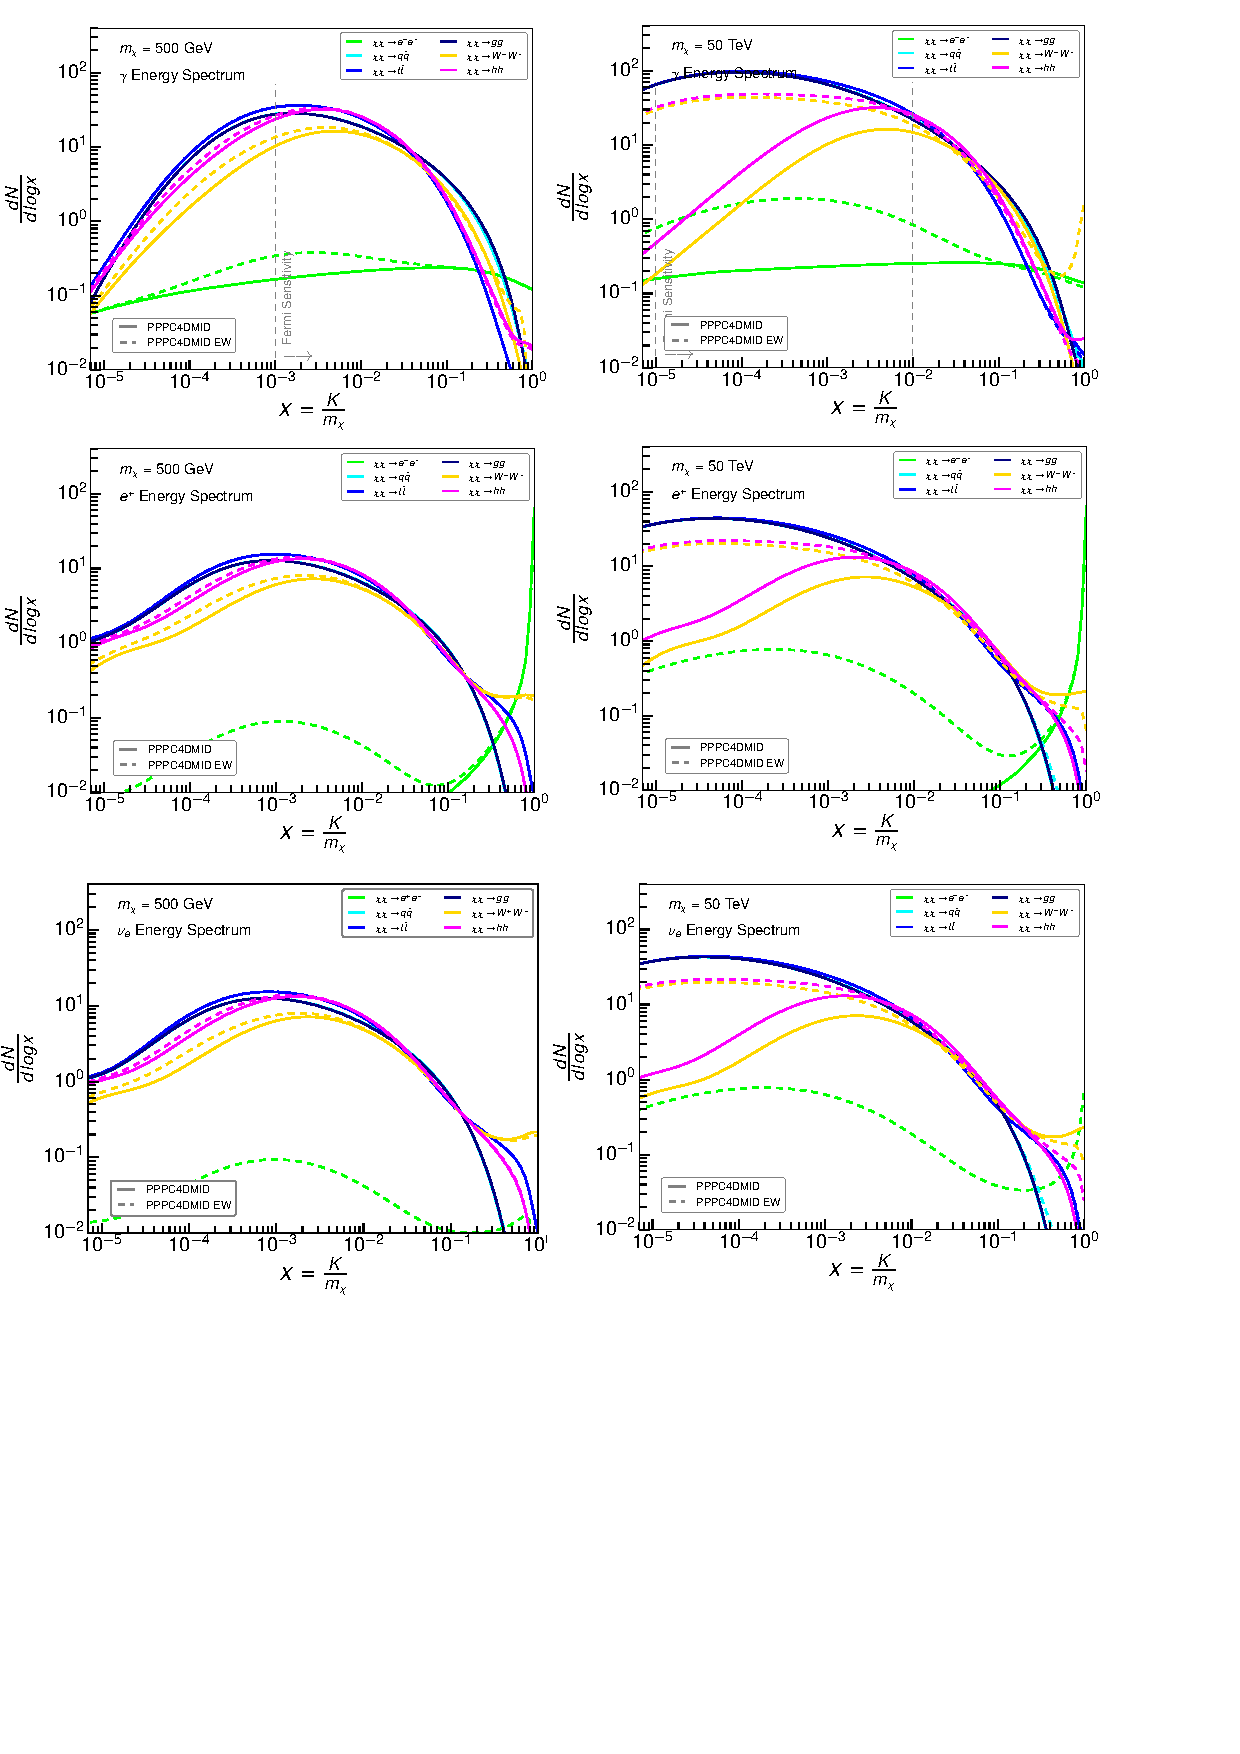
\includegraphics[width=1\textwidth]{Fig/EW_noEW_PPPC.pdf}
\end{center}
\caption{Energy spectra ($\gamma, \e^+, \nu_e$) for $m_{\chi}=$500 GeV (left) and 50 TeV (right) extracted from the \PPPC and \PPPCew tables, from selected annihilation channels.}
\end{figure}







\section*{Acknowledgments}
Thanks

\bibliographystyle{JHEP}
\bibliography{references}

\end{document}
